\documentclass[112pt]{article}
\usepackage{amssymb,amsmath,amsthm}
\usepackage[pdftex]{graphicx}
\usepackage{indentfirst}
\usepackage{tikz}

\addtolength{\jot}{0.5em}
\usepackage[margin=1in]{geometry}

\title{CS124 - Homework 4}
\author{Lucas Freitas}
\date{\today}

\begin{document}

\maketitle

%NUMBER 1
\section*{Problem 1}

Design decision: for the implementation of this algorithm, I used padding to ensure that every possible boundary goes through the same number of comparisons with other $n$-grams.\\

The segmented file that was generated by the TANGO algorithm can be found in the submission folder under the name \texttt{alice\_segmented.txt}.

%NUMBER 2
\section*{Problem 2}

\begin{enumerate}
\item
\texttt{\$ python freitas\_hw3.py -f alice\_tokenized.txt -p alice\_segmented.txt -t 0.95 -n 10}

\begin{verbatim}
precision 0.64873
recall 0.80159

1601 prediction lines used for evaluation
\end{verbatim}

\item
\texttt{\$ python freitas\_hw3.py -f alice\_tokenized.txt -p alice\_segmented.txt -t 0.95 -n 20}

\begin{verbatim}
precision 0.65986
recall 0.80326

1601 prediction lines used for evaluation
\end{verbatim}
\item
As we can see from the data above, the performance goes up when changing the maximum $n$-size from $10$ to $20$, but the increase is not that significant ($\approx 1.7\%$ increase in precision and $\approx 0.2\%$ increase in recall). That shows that having more possible $n$-grams, the algorithm considers the relation of position of word types more carefully, and the segmentation becomes more efficient.\\

That is not that significative, however, for our performance. If we changed from an $n$-gram size of $2$ to $10$, we would see a very significant increase in performance (from $0.42759$ to $0.64873$ in precision and from $0.39285$ to $0.80159$ in recall), since we went from basically ignoring $n$-grams to actually understanding their relation to word segmentation, and considering that in our algorithm. That way, increasing our $n$-gram size will not help much at this point. For $n \ge 10$, we will get values that are extremely close to the maximum performance for our TANGO algorithm, and we should look for other methods, other than changing the maximum $n$-gram size, to increase performance.\\

As a note, using $F$-measure, the performance goes from $\approx 0.717104$ to $\approx 0.724533$, leading to a $\approx 1.04\%$ increase in performance.
\end{enumerate}
\newpage
%NUMBER 3
\section*{Problem 3}
The graph showing the relation between precision and recall can be seen below (although not explicitly shown in the graph, an increase in the threshold leads to higher precision and lower recall).
\begin{center}
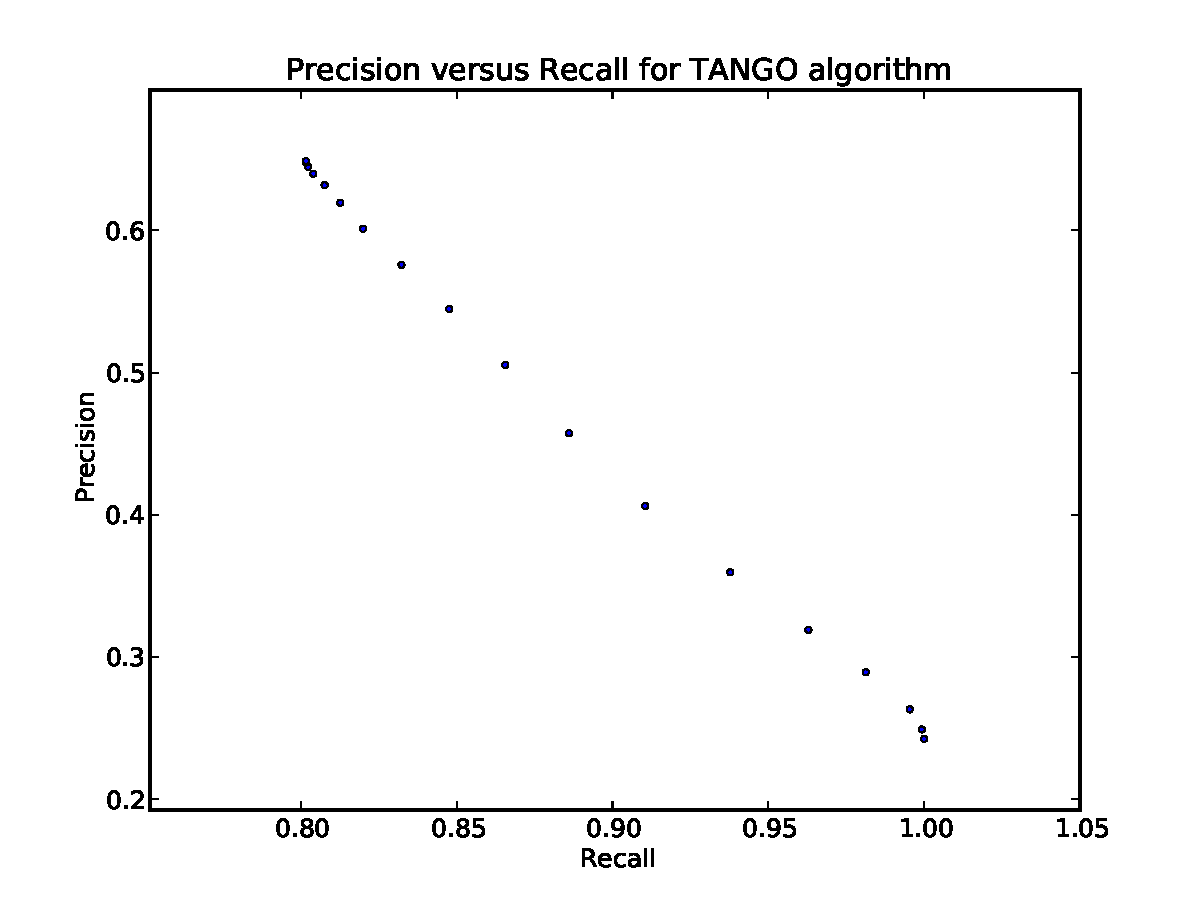
\includegraphics[width=120mm]{graph.pdf}
\end{center}

The graph empirically shows two relations that we expected to happen:
\begin{enumerate}
\item Precision and recall have an inverse relationship. That is simple to see, however, since:
$$Precision = \frac{t_p}{t_p+f_p}$$
$$Recall = \frac{t_p}{t_p+f_n}$$

If we decide to be reckless and guess spaces should be put everywhere, the number of true and false positives will be high. The number of false negatives, however, will probably be very low, and recall will be very close to one, while precision will be low. As we become more careful, the number of false positives would decrease, but the number of false negatives will increase, leading to higher precision and lower recall.

\item
As the threshold increases, precision increases and recall decreases. That is not surprising either: a higher threshold just means that we are being more careful, which leads to higher precision and lower recall according to what we discussed in $(a)$.
\end{enumerate}

%NUMBER 4
\section*{Problem 4}
I would expect the performance of such algorithm to be considerably lower than the TANGO algorithm we used, since although the algorithm would know an approximation of the number of spaces to insert in the text corpus, it wouldn't know the distribution of lengths of words, or the relation between $n$-grams and segmentation.  The algorithm would probably generate word tokens in an intermediate word size compared to possible lengths in the English dictionary word spectrum. \\

TANGO is usually biased into generating shorter word types, which leads to fairly good accuracy because the English language tends to have shorter words (it would be interesting to analyze how well TANGO performs for texts in German), while the algorithm described would be biased towards intermediately-sized words, which are not as common in the English language, and would lead to lower performance.

\end{document}  